\documentclass[aspectratio=169,usenames,dvipsnames]{beamer}

\usepackage{pgf}  
\usepackage{tikz}
\usetikzlibrary{arrows}
\usepgflibrary{shapes.arrows} 
\usetikzlibrary{intersections}
\usetikzlibrary{calc}
\usetikzlibrary{fit}
\usetikzlibrary{automata,positioning}
\usepackage{pgfplots,stackengine}
\usepackage{fontspec}
\usepackage{fancyvrb}
\usepackage{wasysym}
\usepackage{unicode-math}
\usepackage{import}
\usepackage{rotating}
\usepackage{gensymb}
\usepackage{chemfig}
\usepackage{rotating}
\usepackage{booktabs}
\usepackage{pifont}
\usepackage{wrapfig}
\usepackage{mathtools}
\usepackage{graphbox}
\usepackage{epigraph}
\usepackage{listings}
\usepackage{verbatim}
\usepackage{hologo}
\usepackage{wrapfig}
\usepackage[absolute,overlay]{textpos}
\usepackage[euler-digits,euler-hat-accent]{eulervm}
%\logo{\pgfputat{\pgfxy(.45,.5)}{\pgfbox[center]{
\includegraphics[width=1.7cm]{Figures/uu_shadow.pngu}}}}

\usetheme{Copenhagen}
\usecolortheme{beaver}

\definecolor{uured}{RGB}{153,0,0}
\setbeamercolor{block title}{use=structure,fg=white,bg=uured}
\setbeamercolor*{item}{fg=red}

\newcommand{\unilogo}{
  \setlength{\TPHorizModule}{1pt}
  \setlength{\TPVertModule}{1pt}
  \begin{textblock}{1}(26,-10)
   
\includegraphics[height=70pt, align=c]{Figures/uu_shadow.png}
  \end{textblock}
  } 

\pgfmathdeclarefunction{gauss}{2}{%
  \pgfmathparse{1/(#2*sqrt(2*pi))*exp(-((x-#1)^2)/(2*#2^2))}%
}
  
\makeatletter
    \newcases{mycases}{\quad}{%
        \hfil$\m@th\displaystyle{##}$}{$\m@th\displaystyle{##}$\hfil}{\lbrace}{.}
\makeatother

\addtobeamertemplate{frametitle}{}{%
    \unilogo
}
\LetLtxMacro{\oldBlock}{\block}
\LetLtxMacro{\oldEndBlock}{\endblock}
\renewcommand{\block}{\begin{center}\begin{minipage}{0.8\textwidth}\oldBlock}
\renewcommand{\endblock}{\oldEndBlock\end{minipage}\end{center}}
\definecolor{darkpastelgreen}{rgb}{0.01, 0.75, 0.24}

\setlength{\fboxsep}{0pt}

\begin{document}
\graphicspath{{Figures/}}
\setsansfont[ItalicFont = Optima Italic,
             BoldFont = Optima Bold,
             Ligatures=TeX ]
            {Optima Regular}
\setmainfont[ItalicFont = Optima Italic,
             BoldFont = Optima Bold,
             Ligatures=TeX]
            {Optima Regular}
\newfontfamily\commentfont[]{Chalkboard}
\newfontfamily\DejaSans{DejaVuSans.ttf}
\newfontfamily\herculanum[]{Herculanum}
\newfontfamily\timesfont[ItalicFont = Times New Roman Italic]{Times New Roman}
\newcommand{\lmr}{\fontfamily{lmr}\selectfont}
\newfontfamily\zA[Ligatures={Common, Rare}, Variant=1] {Zapfino}
\newfontfamily\zB[Ligatures={Common, Rare}, Variant=2] {Zapfino}
\newfontfamily\zC[Ligatures={Common, Rare}, Variant=3] {Zapfino}
\newfontfamily\zD[Ligatures={Common, Rare}, Variant=4] {Zapfino}
\newfontfamily\zE[Ligatures={Common, Rare}, Variant=5] {Zapfino}
\newfontfamily\zF[Ligatures={Common, Rare}, Variant=6] {Zapfino}
\newfontfamily\zG[Ligatures={Common, Rare}, Variant=7] {Zapfino}
\renewcommand\UrlFont{\color{blue}}
\renewcommand\thefootnote{\textcolor{uured}{\arabic{footnote}}}
\setbeamercolor{alerted text}{fg=uured}
\lstset{basicstyle=\ttfamily\scriptsize, frame=single }
\newcommand{\TikZ}{{\lmr Ti\textit{k}Z}}

\title{An introduction to Apache Spark}   
\author{Jonathan Alvarsson} 
%\titlegraphic{\vfill\includegraphics[width=18em]{Figures/ORN_large.png}}
\date{\today} 

\setbeamertemplate{background}{%
    \parbox[c][\paperheight]{\paperwidth}{%
        \vfill
        \hfill
        
\includegraphics[height=0.65\textheight]{Figures/sigill.png}
    }   
}
\begin{frame}[plain]
\unilogo\titlepage
\begin{tikzpicture}[remember picture,overlay]
\tikz[remember picture, overlay] \fill[uured] (current page.north west) rectangle ++(\paperwidth,-0.5cm);
\end{tikzpicture}%
\end{frame}

\setbeamertemplate{background}{}
\renewcommand{\unilogo}{
  \setlength{\TPHorizModule}{1pt}
  \setlength{\TPVertModule}{1pt}
  \begin{textblock}{1}(0,0)
   
\includegraphics[height=27pt, align=c]{Figures/uu.png}
  \end{textblock}
  } 
\section{Background}
    \begin{frame}
    \frametitle{Outline}
    \begin{minipage}{0.25\textwidth}
    \mbox{}
    \end{minipage}
    \begin{minipage}{0.6\textwidth}
    \tableofcontents[hideallsubsections]
    \end{minipage}
    \end{frame}

    \subsection{LISP}
\setbeamertemplate{background}{%
    \parbox[c][\paperheight]{\paperwidth}{%
        \vskip -0.1 ex \hskip -1 em
        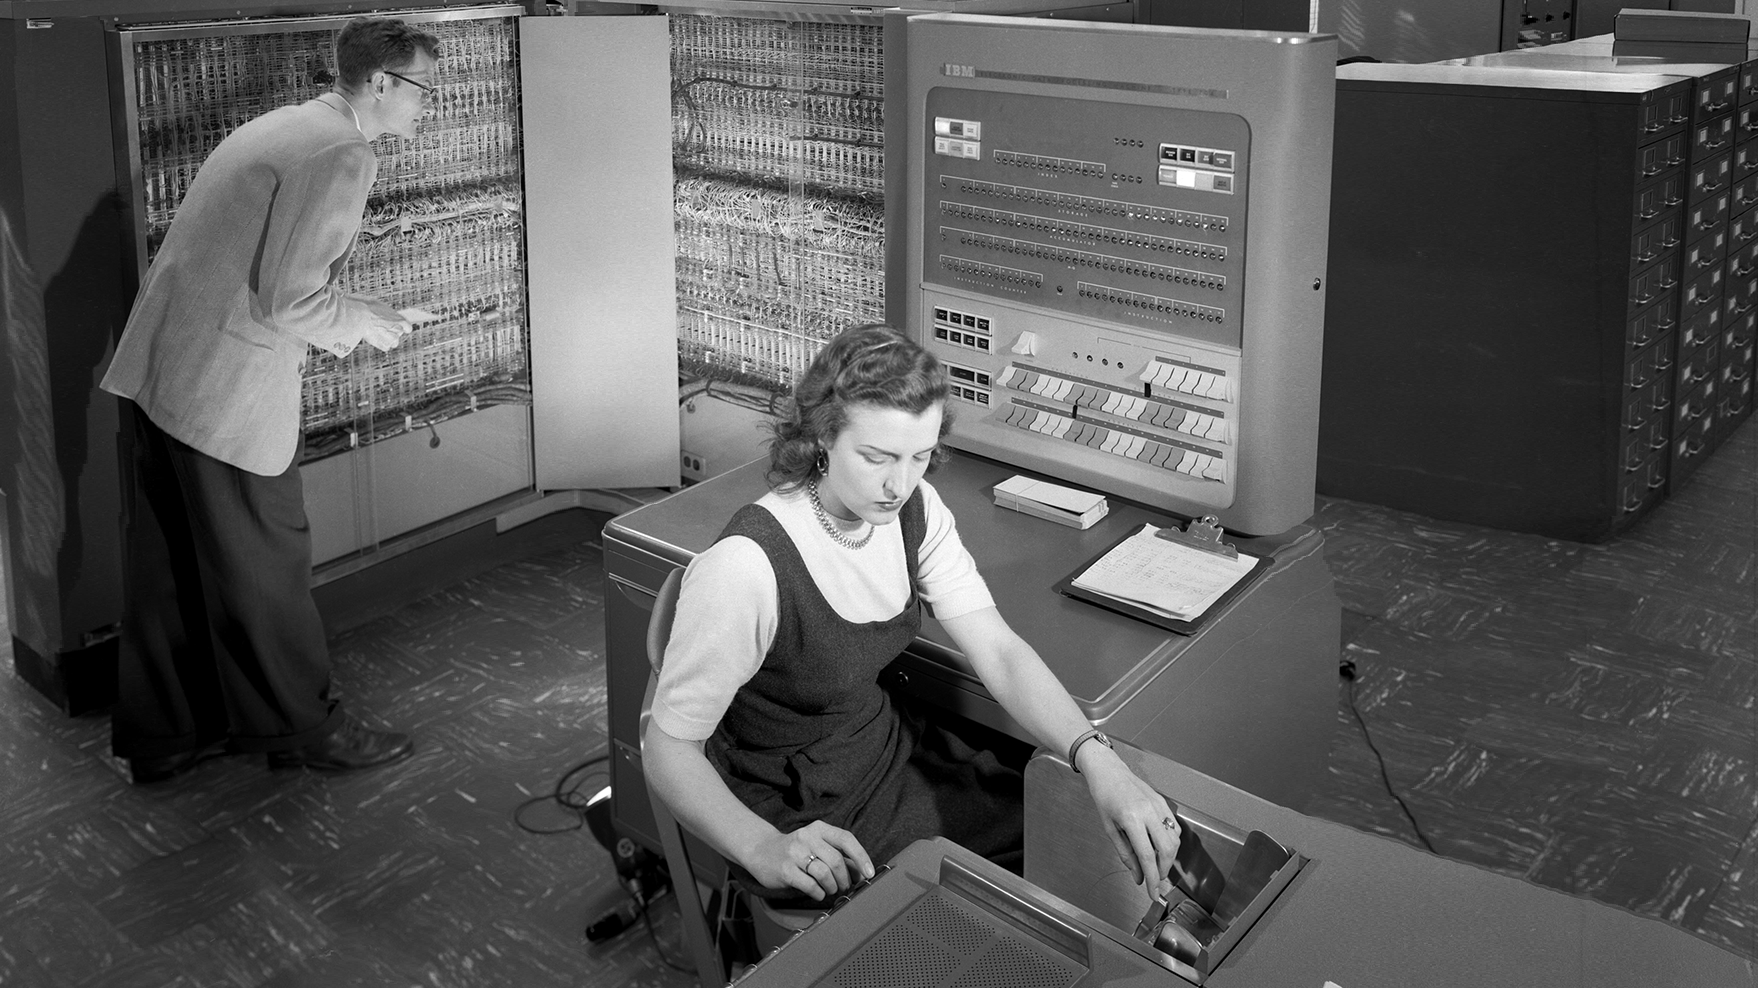
\includegraphics[width=1.05\paperwidth]{Figures/LISP.png}
    }   
}
\begin{frame}[plain]
        %\vskip -20 ex
    %\Large\qquad\qquad\qquad\color{black} {\zA In the beginning there was} \\
    %\Huge LISP
\hfill        {\small\color{white}IBM 704 Computer in 1957}
\vfill\vfill\vfill\vfill\vfill
\begin{minipage}[c]{0.5\textwidth}
        \pause
        \oldBlock{\zA "In the beginning there was":}
        \begin{center}
        \vspace*{2ex}
        \Huge LISP
        \vspace*{1ex}
        \end{center}
        \oldEndBlock
\end{minipage}\hfill


\end{frame}
\setbeamertemplate{background}{}
    \begin{frame}
        \frametitle{LISP}
        \framesubtitle{LISt Processor}
            \begin{center}\texttt{(print "Hello, World!")}\end{center}
        \begin{block}{LISP}
            \begin{itemize}
                \item created in 1958
                \item is the second-oldest high-level programming language in widespread use today
            \end{itemize}
        \end{block}

    \end{frame}
    \begin{frame}[fragile]
        \frametitle{LISP}
        \framesubtitle{LISt Processor}
\begin{minipage}{0.42\textwidth}
\raggedright
LISP is a powerful, but in my opinion, somewhat special language. Here is an example\footnotemark calculating the factorial of a number {\small (directly from Wikipedia)}:
\begin{lstlisting}
(defun factorial (n)
    (if (= n 0) 1
        (* n (factorial (- n 1)))))
\end{lstlisting}
\end{minipage}
\hfill
\uncover<2->{
\begin{minipage}{0.55\textwidth}
\centering
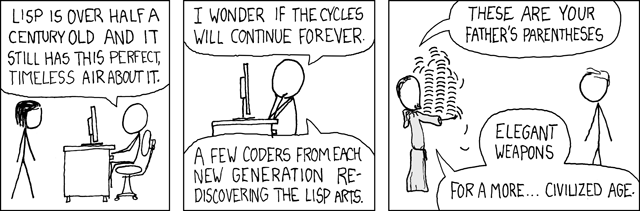
\includegraphics[width=1\textwidth]{Figures/lisp_cycles.png}
\small \texttt{https://xkcd.com/297/}
\end{minipage}}
\footnotetext{You do \alert{\underline{not}} need to learn LISP in this course}
    \end{frame}

    \subsection{Map and Reduce}

    \begin{frame}
        \frametitle{Map and Reduce}
        \color{lightgray}
        \begin{center}
            \only<1->{\only<1>{\color{black}}So, why do I talk so much about LISP?}
        \end{center}
        \begin{center}
            \only<2->{\only<2>{\color{black}}It's because its list-based structure lent itself well for \texttt{map} and \texttt{reduce}}
        \end{center}
        \begin{center}
            \only<3->{\only<3>{\color{black}}Which later gave rise to the MapReduce programming model}
        \end{center}
        \begin{center}
            \only<4->{\only<4>{\color{black}}but first, let's talk about \texttt{map} and \texttt{reduce}\ldots}
        \end{center}
    \end{frame}

    \begin{frame}[fragile]
        \frametitle{Map and Reduce}
        \framesubtitle{Map}

            \begin{block}{Map}
                \texttt{map} is a higher-order function that applies a given
                function to each element of, \textit{e.g.}, a list. It can also
                be called \texttt{apply-to-all}.
            \end{block}
            \begin{uncoverenv}<2->
            \begin{block}{Example: \hfill \small(Python)}
            \begin{center}
            \begin{minipage}{0.8\linewidth}
            \begin{lstlisting}
square = lambda x:x*x
a = [1,2,3,4]
list(map(square, a))
            \end{lstlisting}
            $\Rightarrow$ \texttt{[1, 4, 9, 16]}
            \end{minipage}
            \end{center}
            \end{block}
            \end{uncoverenv}
        
    \end{frame}
    
    \begin{frame}[fragile]
        \frametitle{Map and Reduce}
        \framesubtitle{Reduce}

            \begin{block}{Reduce}
                \texttt{reduce} is a higher-order function that by using a
                given function combines the part of, \textit{e.g.}, a list into
                a return value.
            \end{block}
            \begin{uncoverenv}<2->
            \begin{block}{Example: \hfill \small(Python)}
            \begin{center}
            \begin{minipage}{0.8\linewidth}
            \begin{lstlisting}
from functools import reduce
sum = lambda a,b:a+b
a = [1,2,3,4]
reduce(sum,a)
            \end{lstlisting}
            $\Rightarrow$ 10
            \end{minipage}
            \end{center}
            \end{block}
            \end{uncoverenv}
    \end{frame}

    \subsection{MapReduce}
    \begin{frame}
        \frametitle{MapReduce frameworks}
        \framesubtitle{Parallelisation}
        \begin{block}{MapReduce frameworks are parallel}
        Since each step in Map and Reduce is separate it lends itself well to
        parallelisation. The idea behind MapReduce frameworks is to run in
        massively parallel ways.
        \end{block}
    \end{frame}
       
    \begin{frame}
        \frametitle{MapReduce frameworks}
        \framesubtitle{Parallelisation}
        \begin{block}{Apache Hadoop}
        \begin{wrapfigure}[2]{r}{0.45\textwidth}
        \vspace{-1.2\baselineskip}
        
\includegraphics[width=1\linewidth]{figures/hadoop.png}
        \end{wrapfigure}
        Apache Hadoop is an example of a MapReduce framework that:
        \begin{itemize}
            \item Was released in 2006
            \item Works by loading things from disk, performing map and reduce operations and then writing back to disk.
            \item Can use relatively cheap computers to run things in parallel
            \item Has relatively hard APIs to code against while doing the map and reduce operations
        \end{itemize}
        \end{block}
    \end{frame}


\section{Spark}
    \begin{frame}
        \frametitle{Spark}
        \framesubtitle{``a unified analytics engine for large-scale data processing''}
        \begin{block}{Apache Spark}
        \begin{wrapfigure}[3]{r}{0.35\textwidth}
        \vspace{-1\baselineskip}
        
\includegraphics[width=0.9\linewidth]{figures/Spark.png}\hfill
        \end{wrapfigure}
        In 2014 Spark was released, in a way as a sort of response to Hadoop. Spark:
        \begin{itemize}
            \item Keeps things in memory and is thus faster than Hadoop
        \end{itemize}\vspace{-4pt}

        \begin{itemize}
            \item Has friendly APIs for Python, Scala and to some degree R
            \item Has better support for machine learning than Hadoop
            \item Requires relatively expensive computers to run because it
            needs huge amounts of RAM if it is to benefit from keeping all data
            in memory.
        \end{itemize}
        \end{block}
    \end{frame}

    \begin{frame}
        \frametitle{Spark}
        \framesubtitle{``a unified analytics engine for large-scale data processing''}
        \begin{block}{Apache Spark}
        \begin{center}
            \only<1>{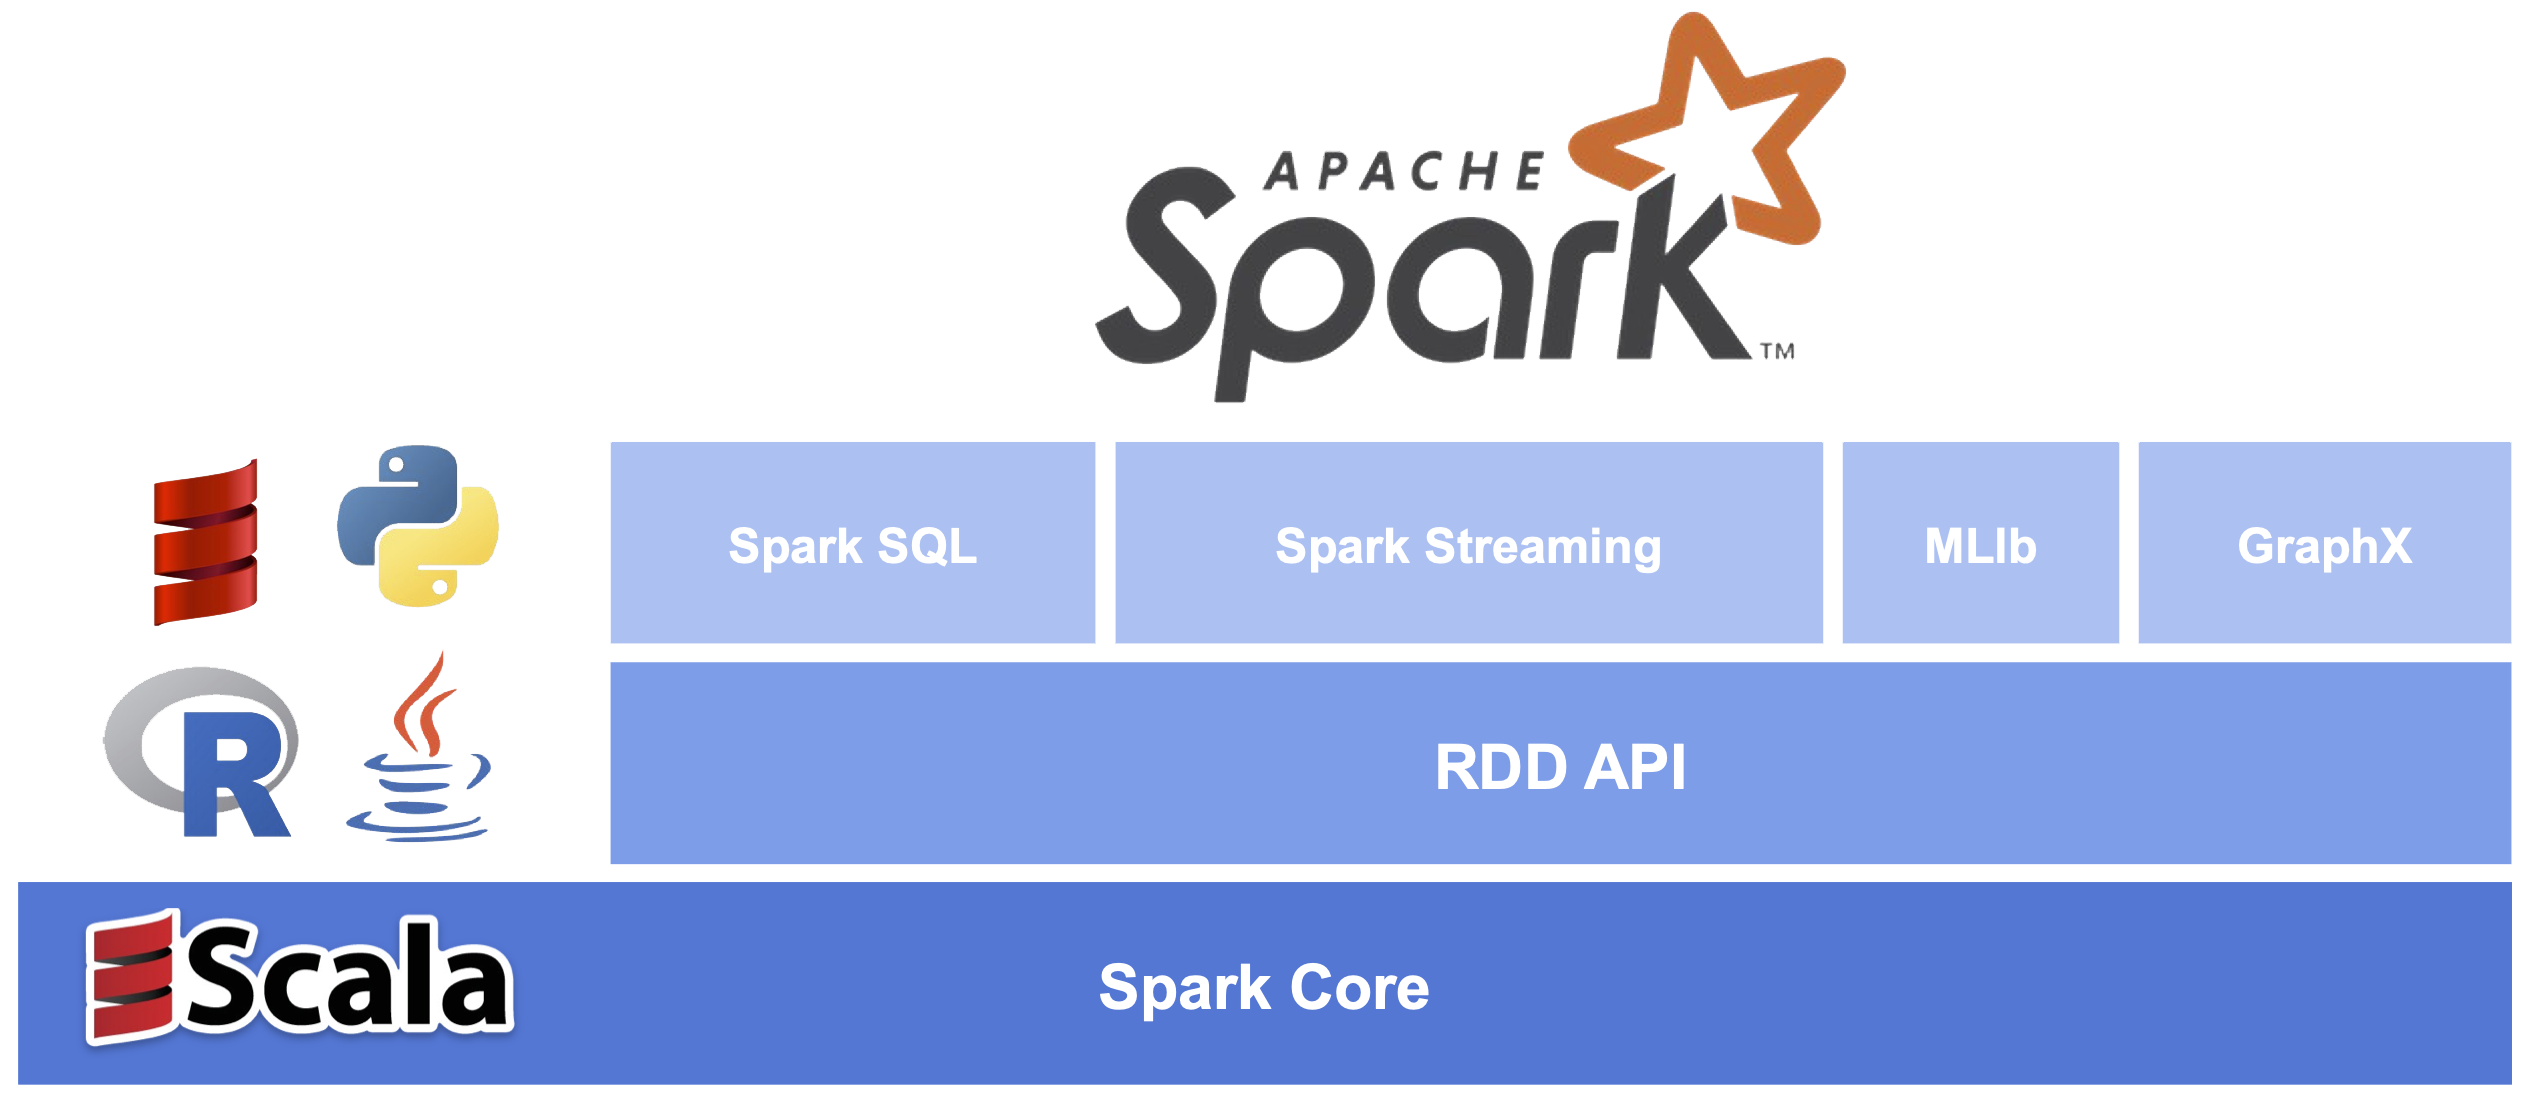
\includegraphics[width=0.9\textwidth]{figures/spark-overview.png}}
            \only<2>{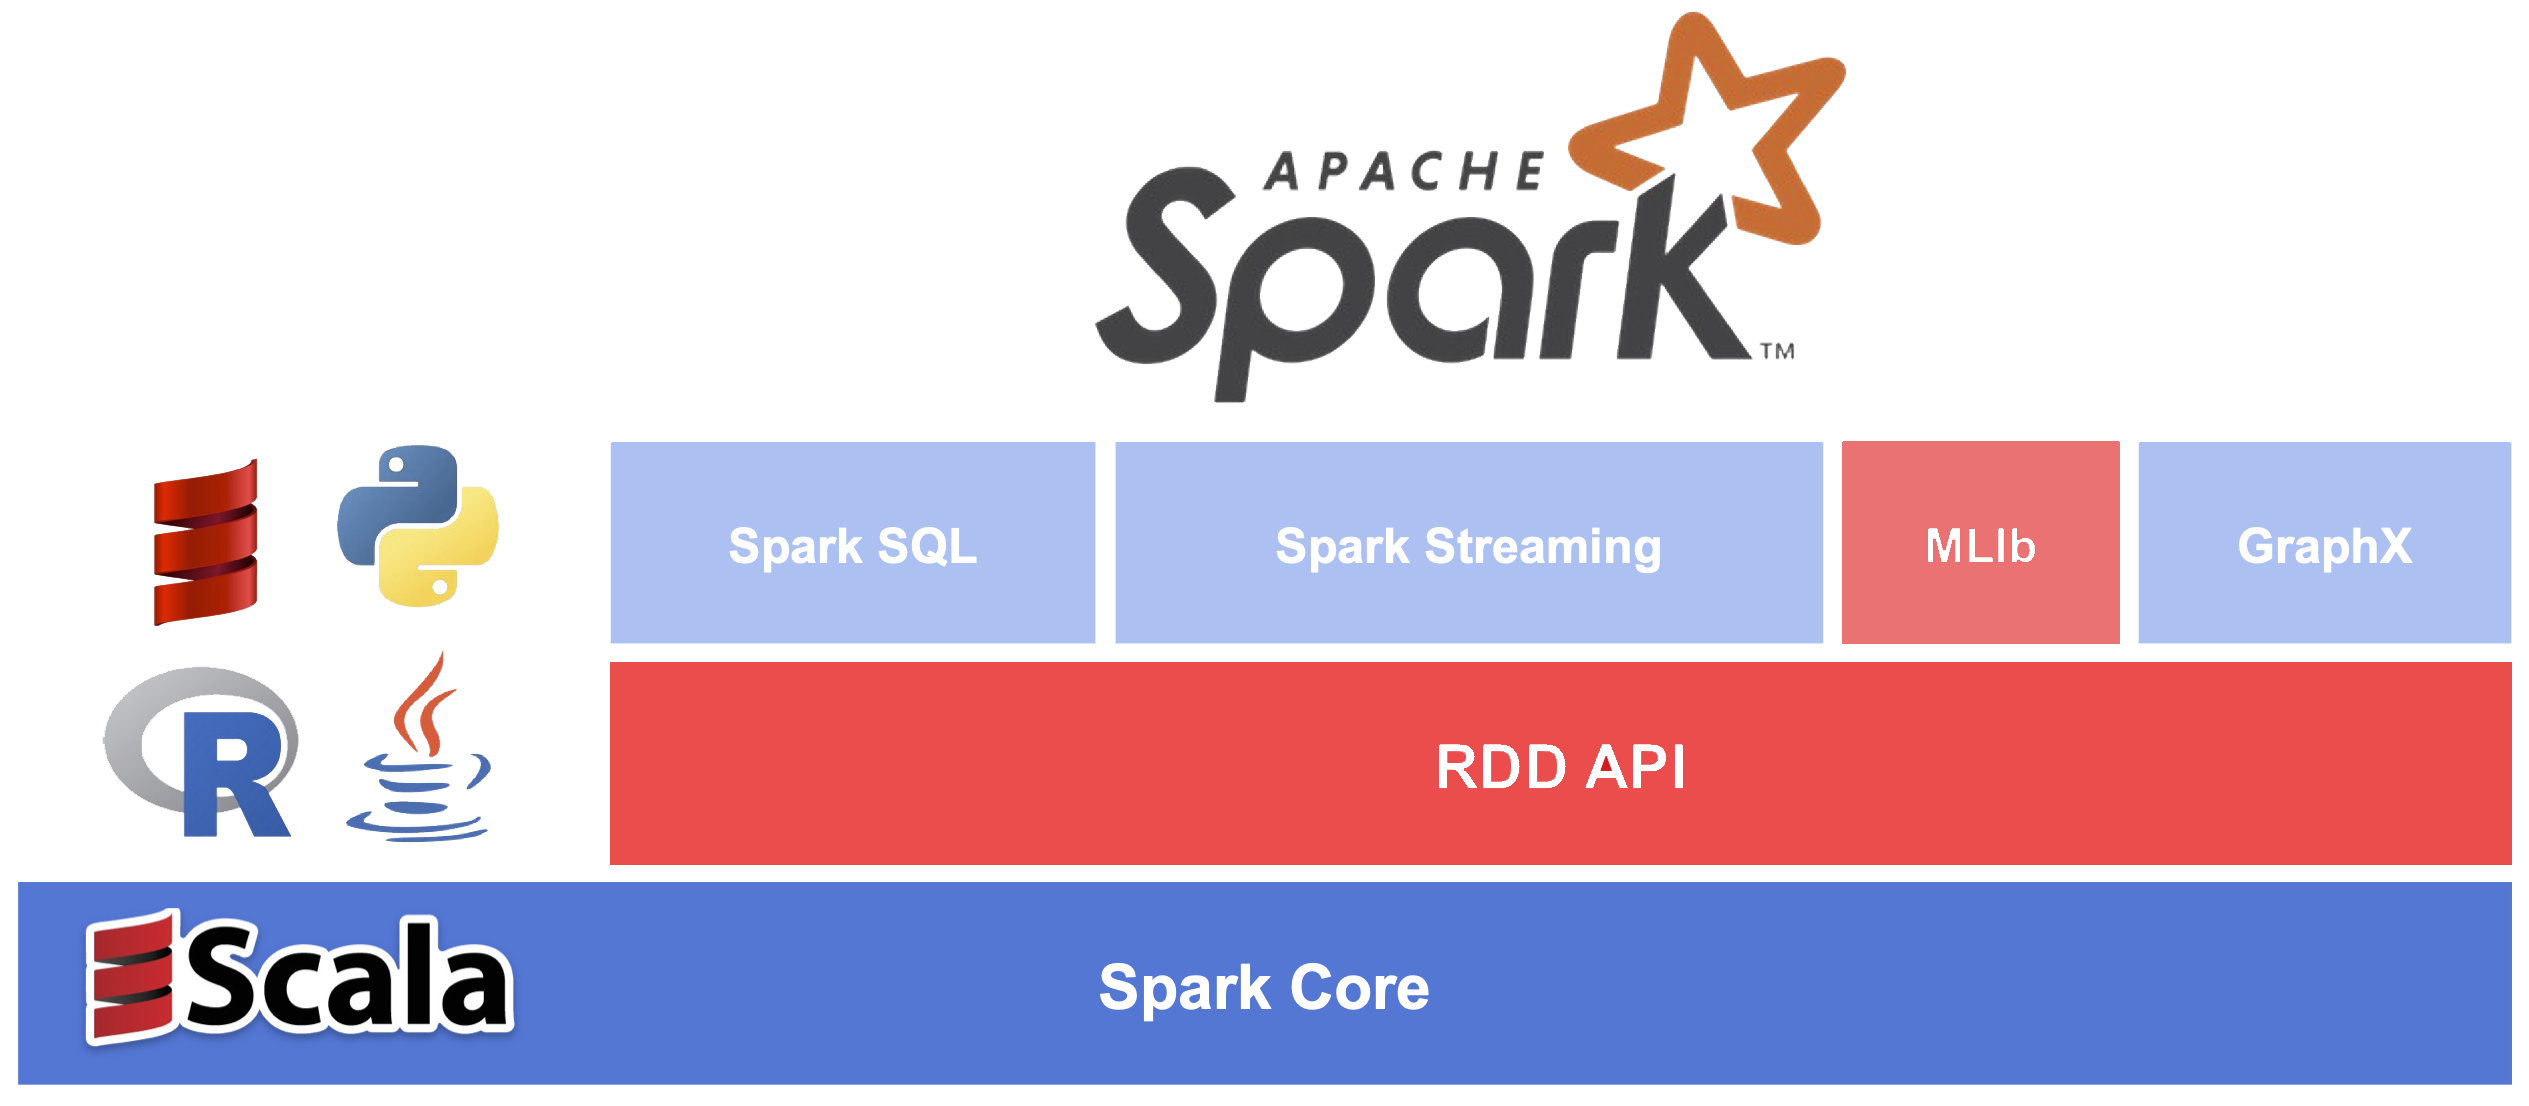
\includegraphics[width=0.9\textwidth]{figures/spark-overview-select.png}}
        \end{center}
        \end{block}
    \end{frame}

    \subsection{Architecture}
        \begin{frame}
            \frametitle{Spark}
            \framesubtitle{Architecture}
            \begin{block}{Spark Architecture}
            \begin{center}
            \begin{tikzpicture}[node distance=0]
        \node (context)  [draw,minimum height=.5cm,minimum width = .5cm, node distance = 55 pt]{Spark Context};
        \node (manager)  [draw,minimum height=.5cm,minimum width = .5cm, right of = context, node distance = 10 em]{Cluster Manager};
        \node (worker1)  [draw,minimum height=.5cm,minimum width = .5cm, right of = manager, node distance = 10 em,  yshift=8ex]{Executor};
        \node (worker2)  [draw,minimum height=.5cm,minimum width = .5cm, right of = manager, node distance = 10 em             ]{Executor};
        \node (worker3)  [draw,minimum height=.5cm,minimum width = .5cm, right of = manager, node distance = 10 em, yshift=-8ex]{Executor};

        \node (contextT) [above of = context, node distance=3ex] {\small\commentfont Driver code};
        \node (worker1T) [above of = worker1, node distance=3ex] {\small\commentfont Worker};
        \node (worker2T) [above of = worker2, node distance=3ex] {\small\commentfont Worker};
        \node (worker3T) [above of = worker3, node distance=3ex] {\small\commentfont Worker};

        \draw [->, shorten <=4pt, shorten >=4pt] (context) to (manager);
        \draw [->, shorten <=4pt, shorten >=4pt, out=10, in=-170] (manager) to (worker1);
        \draw [->, shorten <=4pt, shorten >=4pt, out=0, in=180]  (manager) to (worker2);
        \draw [->, shorten <=4pt, shorten >=4pt, out=-10, in=170] (manager) to (worker3);

            \end{tikzpicture}
            \vspace{1ex}
            \end{center}
            \end{block}

        \end{frame}

    \subsection{RDD}
        \begin{frame}
            \frametitle{Spark}
            \framesubtitle{RDD -- ``A read-only collection of records partitioned through the nodes in the cluster''}
            \begin{block}{RDD -- Resilient Distributed Dataset}
                When coding in Spark you work with RDDs. They are:
                \begin{itemize}
                    \item Immutable 
                    \item Distributed and partitioned in the cluster
                    \item Scalable and fault tolerant
                    \item Created from stored data or by transforming another RDD
                \end{itemize}
            \end{block}
        \end{frame}
        
        \begin{frame}
            \frametitle{Spark}
            \framesubtitle{RDD -- ``A read-only collection of records partitioned through the nodes in the cluster''}
            \begin{block}{Transformations}
                A transformation 
                \begin{itemize}
                    \item creates a \alert{new RDD} from an old RDD
                    \item is evaluated \alert{lazily}
                \end{itemize}
            \end{block}
            \begin{block}{Actions}
                An action 
                \begin{itemize}
                    \item \alert{saves data} to file system or \alert{returns data} to driver program
                    \item \alert{blocks} while being evaluated
                \end{itemize}
            \end{block}
        \end{frame}

    \subsection{Dataframe}
        \begin{frame}
            \frametitle{Spark}
            \framesubtitle{Dataframe}
            \begin{block}{Dataframe}
                When doing machine learning with Spark we will work a lot with
                dataframes. A dataframe consists of rows and columns.
            \end{block}
        \end{frame}

\section{Example}
        \begin{frame}
            \frametitle{Spark}
            \framesubtitle{Example}
            \begin{center}
                Now, let's look at an example!
            \end{center}
        \end{frame}

\subsection{Word counting}
    \begin{frame}[fragile]
        \frametitle{Example}
        \framesubtitle{Word counting}
        \begin{center}

        \begin{minipage}{0.8\textwidth}
\begin{lstlisting}[escapechar={|}, title=wordcount.py]
|\only<1>{\color{black}}{\only<2>{\color{gray}}from pyspark.sql import SparkSession |

|\only<1>{\color{black}}{\only<2>{\color{Orchid}}spark = SparkSession.builder.appName("SimpleApp").getOrCreate()|
|\only<1>{\color{black}}{\only<2>{\color{Orchid}}sc = spark.sparkContext|

|\only<1>{\color{black}}{\only<2>{\color{NavyBlue}}rdd0 = sc.textFile("foo.txt")|

|\only<1>{\color{black}}{\only<2>{\color{NavyBlue}}rdd1 = rdd0.flatMap( lambda line : line.split(" ") )|
|\only<1>{\color{black}}{\only<2>{\color{NavyBlue}}rdd2 = rdd1.map( lambda word : (word,1) )|
|\only<1>{\color{black}}{\only<2>{\color{NavyBlue}}rdd3 = rdd2.reduceByKey( lambda a,b : (a + b) )|

|\only<1>{\color{black}}{\only<2>{\color{BrickRed}}print(rdd3.collect())|
\end{lstlisting}
\end{minipage}
\end{center}
    \end{frame}

    \begin{frame}[plain]
    \hspace*{-1em}
            \begin{tikzpicture}[node distance= 25 pt]
        \only<1>{
        \node (txt)  [fill={rgb:purple,1;white,4}, draw,minimum height=.5cm,minimum width = .5cm, node distance = 55 pt]{foo bar foo bar buzz};
        \node [above of = txt, node distance = 14 pt] {\small\commentfont foo.txt };
        }

        \only<6>{
        \node (txt)  [fill={rgb:purple,1;white,4}, draw,minimum height=.5cm,minimum width = .5cm, node distance = 55 pt]{foo bar foo bar buzz};
        \node [above of = txt, node distance = 14 pt] {\small\commentfont foo.txt };
        }
        
        \uncover<2-5>{
        \node (txt)  [fill={rgb:purple,1;white,15}, draw,minimum height=.5cm,minimum width = .5cm, node distance = 55 pt]{foo bar foo bar buzz};
        \node [above of = txt, node distance = 14 pt] {\small\commentfont foo.txt };
        }
        
        \only<2->{
        \node (rdd0)  [fill={rgb:purple,1;white,4}, below of = txt, draw,minimum height=.5cm,minimum width = .5cm, node distance = 55 pt]{"foo bar foo bar buzz"};
        \node [above of = rdd0, node distance = 14 pt] {\small\commentfont rdd0 };
        \draw [->, shorten <=4pt, shorten >=4pt,out=-35, in=35] (txt) to node[right]
              {\color{NavyBlue}\small\texttt{rdd0 = sc.textFile("foo.txt")}} (rdd0);
        }

        \uncover<3->{
        \node (rdd0)  [fill={rgb:purple,1;white,15}, below of = txt, draw,minimum height=.5cm,minimum width = .5cm, node distance = 55 pt]{"foo bar foo bar buzz"};
        \node [above of = rdd0, node distance = 14 pt] {\small\commentfont rdd0 };
        \draw [->, shorten <=4pt, shorten >=4pt,out=-35, in=35] (txt) to node[right]
              {\color{NavyBlue!40!white}\small\texttt{rdd0 = sc.textFile("foo.txt")}} (rdd0);
        }
        
        \only<3->{
        \node (rdd1)  [fill={rgb:purple,1;white,4}, below of = rdd0, draw,minimum height=.5cm,minimum width = .5cm, node distance = 55 pt]{"foo", "bar", "foo", "bar", "buzz"};
        \node [above of = rdd1, node distance = 14 pt] {\small\commentfont rdd1 };
        \draw [->, shorten <=4pt, shorten >=4pt,out=-35, in=35] (rdd0) to node[right]
              {\color{NavyBlue}\small\texttt{rdd1 = rdd0.flatMap( lambda line : line.split(" ") )}} (rdd1);
        }

        \uncover<4->{
        \node (rdd1)  [fill={rgb:purple,1;white,15}, below of = rdd0, draw,minimum height=.5cm,minimum width = .5cm, node distance = 55 pt]{"foo", "bar", "foo", "bar", "buzz"};
        \node [above of = rdd1, node distance = 14 pt] {\small\commentfont rdd1 };
        \draw [->, shorten <=4pt, shorten >=4pt,out=-35, in=35] (rdd0) to node[right]
              {\color{NavyBlue!40!white}\small\texttt{rdd1 = rdd0.flatMap( lambda line : line.split(" ") )}} (rdd1);
        }
        
        \only<4->{
        \node (rdd2)  [fill={rgb:purple,1;white,4}, below of = rdd1, draw,minimum height=.5cm,minimum width = .5cm, node distance = 55 pt]
                      {("foo", 1), ("bar", 1), ("foo", 1), ("bar", 1), ("buzz", 1)};
        \node [above of = rdd2, node distance = 14 pt] {\small\commentfont rdd2 };
        \draw [->, shorten <=4pt, shorten >=4pt,out=-35, in=35] (rdd1) to node[right]
              {\color{NavyBlue}\small\texttt{rdd2 = rdd1.map( lambda word : (word,1) )}} (rdd2);
        }
        
        \uncover<5->{
        \node (rdd2)  [fill={rgb:purple,1;white,15}, below of = rdd1, draw,minimum height=.5cm,minimum width = .5cm, node distance = 55 pt]
                      {("foo", 1), ("bar", 1), ("foo", 1), ("bar", 1), ("buzz", 1)};
        \node [above of = rdd2, node distance = 14 pt] {\small\commentfont rdd2 };
        \draw [->, shorten <=4pt, shorten >=4pt,out=-35, in=35] (rdd1) to node[right]
              {\color{NavyBlue!40!white}\small\texttt{rdd2 = rdd1.map( lambda word : (word,1) )}} (rdd2);
        }
        
        \only<5->{
        \node (rdd3)  [fill={rgb:purple,1;white,4}, below of = rdd2, draw,minimum height=.5cm,minimum width = .5cm, node distance = 55 pt]
                      {("foo", 2), ("bar", 2), ("buzz", 1)};
        \node [above of = rdd3, node distance = 14 pt] {\small\commentfont rdd3 };
        \draw [->, shorten <=4pt, shorten >=4pt,out=-35, in=35] (rdd2) to node[right]
              {\color{NavyBlue}\small\texttt{rdd3 = rdd2.reduceByKey( lambda a,b : (a + b) )}} (rdd3);
        }
        
        \uncover<6->{
        \node (rdd3)  [fill={rgb:purple,1;white,4}, below of = rdd2, draw,minimum height=.5cm,minimum width = .5cm, node distance = 55 pt]
                      {("foo", 2), ("bar", 2), ("buzz", 1)};
        \node [above of = rdd3, node distance = 14 pt] {\small\commentfont rdd3 };
        \draw [->, shorten <=4pt, shorten >=4pt,out=-35, in=35] (rdd2) to node[right]
              {\color{NavyBlue!40!white}\small\texttt{rdd3 = rdd2.reduceByKey( lambda a,b : (a + b) )}} (rdd3);
         
        \draw [->, shorten <=4pt, shorten >=4pt,out=15, in=-15, line width=1mm, opacity=0.85, color={rgb:purple,1;white,1}] (rdd3) to node[right,text width=6cm]
              {\commentfont \Large Now we have made a word count of the original file} (txt);
        }
            \end{tikzpicture}
    \end{frame}

\begin{frame}[fragile]
        \frametitle{Example}
        \framesubtitle{Word counting}
        
\end{frame}

\setbeamertemplate{background}{%
    \parbox[c][\paperheight]{\paperwidth}{%
        \vskip -8 ex \hskip -2 em
        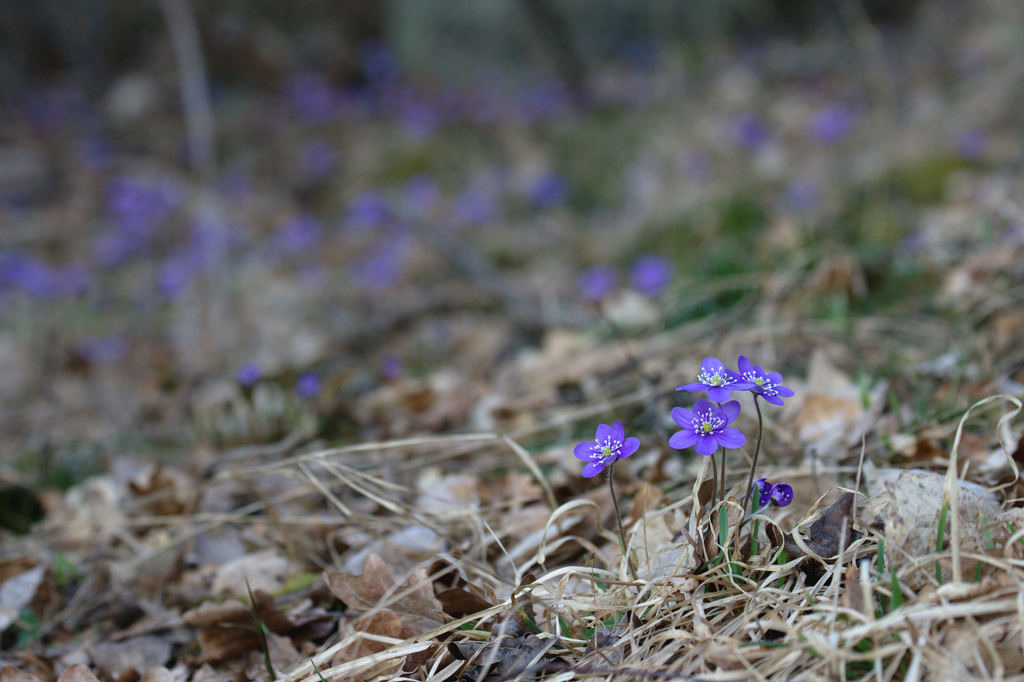
\includegraphics[height=1.5\paperheight]{Figures/blasippa.jpg}
    }   
    \parbox[c][\paperheight]{\paperwidth}{%
        \vskip 25 ex \hskip -40 em
        \color{white}\fbox{
\includegraphics[height=0.37\paperheight]{Figures/me.jpg}}
    }   
}
\begin{frame}[plain]
    \vfill\hfill{\Huge\qquad\color{white} \zB Thank \zC you}\hfill\hfill\hfill\vfill
\end{frame}
\setbeamertemplate{background}{}
\end{document}
